\chapter{Evaluation}




\begin{itemize}
    \item Top k: predicted class is within the top k predictions
    \item calculation for top k: 
    \[\frac{\binom{NUM\_CLASSES - 1}{k - 1}}{\binom{NUM\_CLASSES}{k}} = \frac{k}{NUM\_CLASSES}\]
    \item for the floor with most files: NUM\_CLASSES = 4795
    \item Probabilities, see \cref{fig:random_accuracies_4795_classes}
\end{itemize}

\begin{figure}[h!]
    \centering
    \includegraphics*[scale=0.8]{images/random_accuracies_4795_classes.png}
    \caption{Probabilities that the predicted class falls within the top k randomly selected classes.}
    \label{fig:random_accuracies_4795_classes}
\end{figure}



\begin{figure}[h!]
    \centering

    \begin{subfigure}[b]{0.45\textwidth}
        \centering
        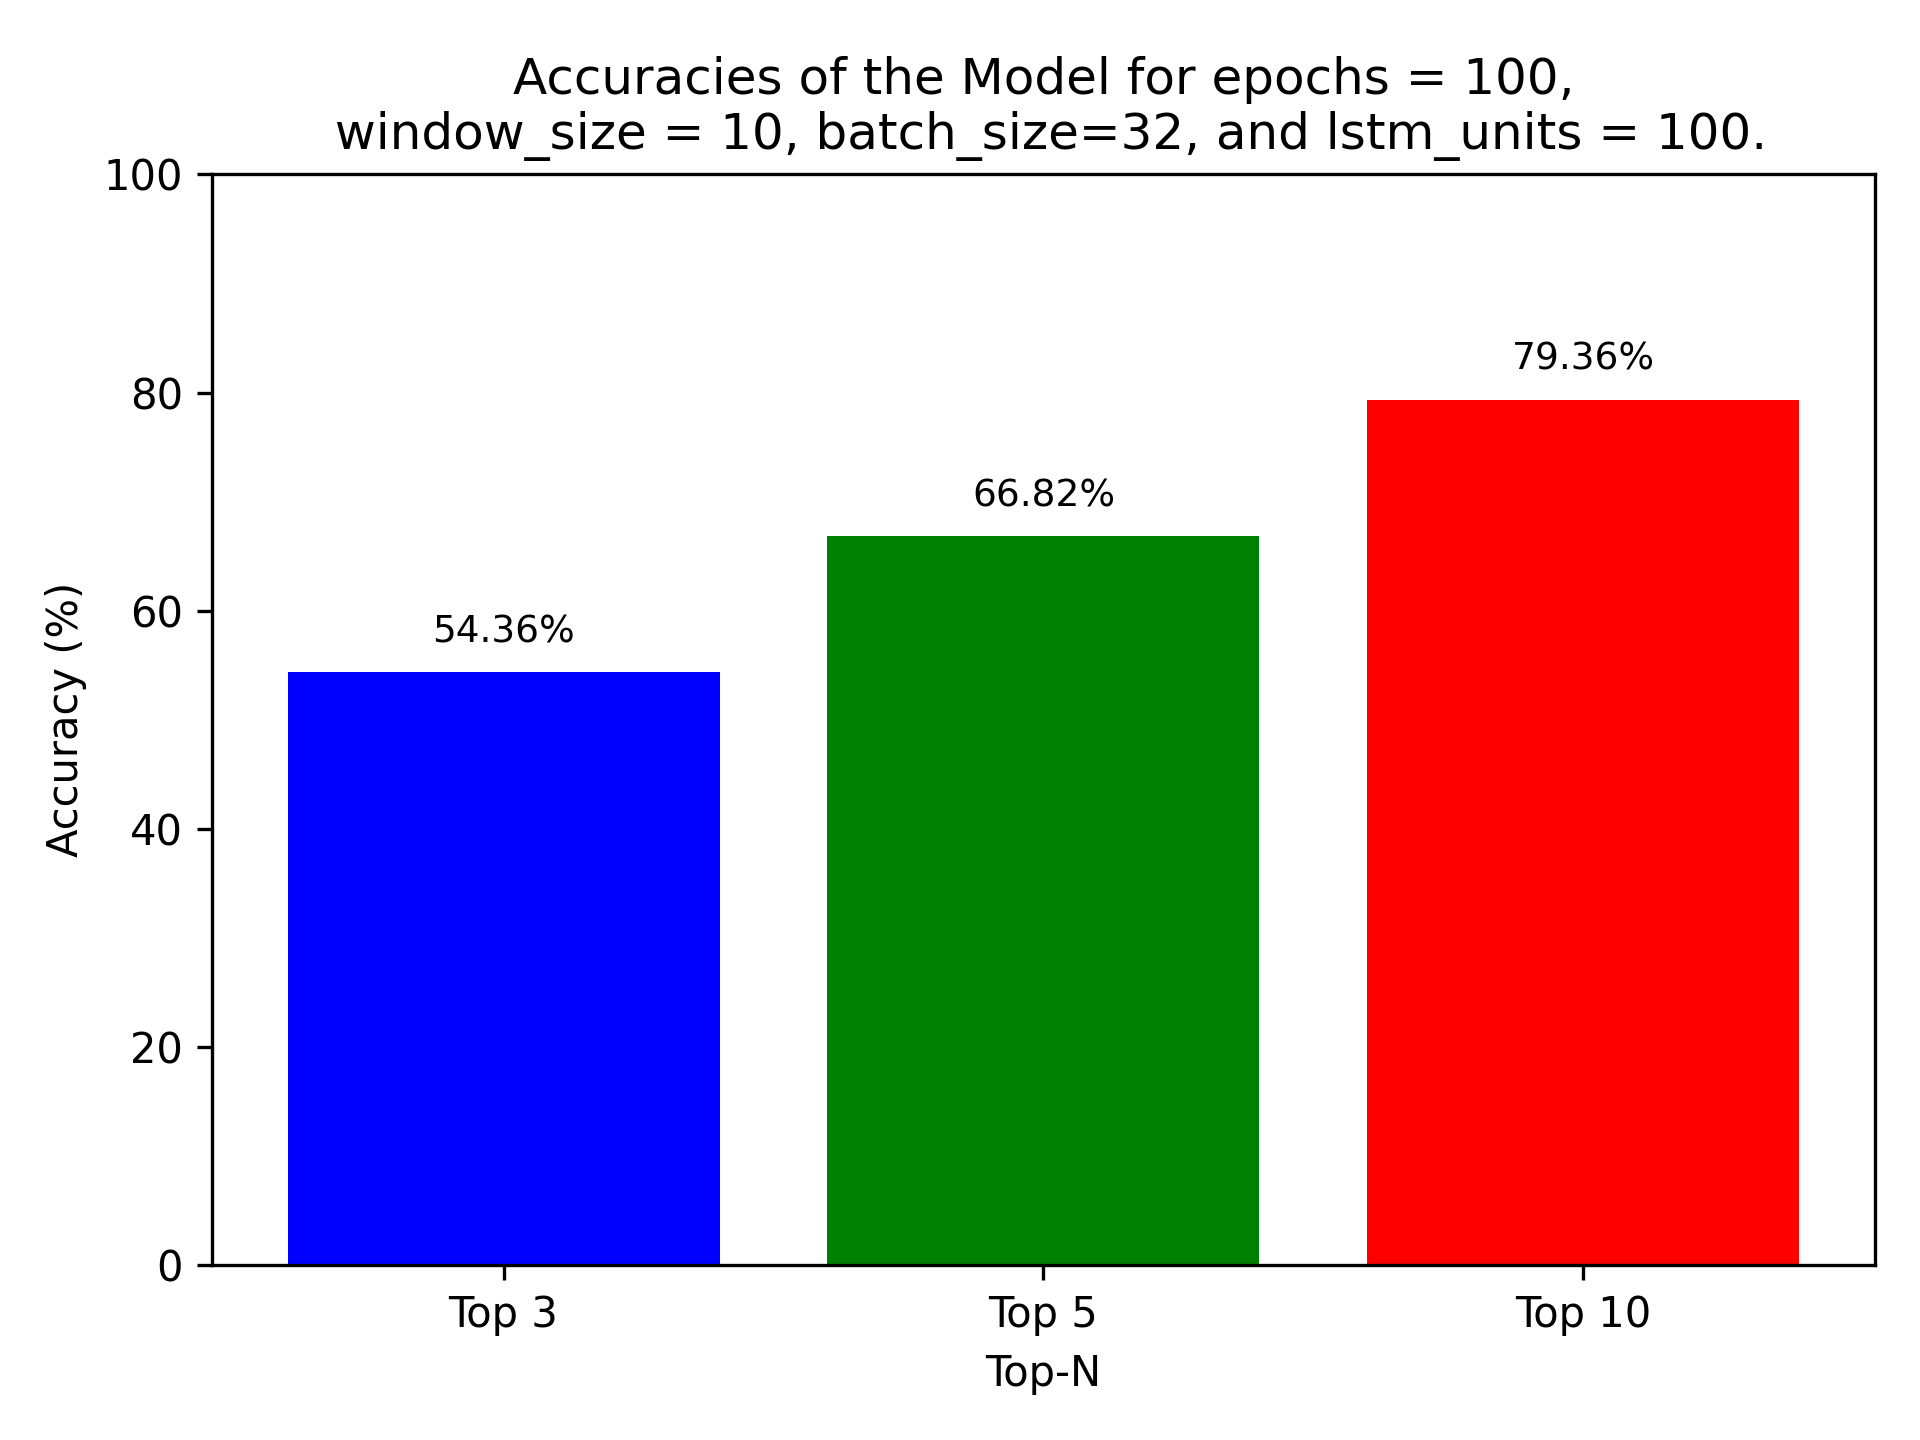
\includegraphics[scale=0.5]{images/accuracy_epochs_100_window_10_batch_32_lstm_100.png}
    \end{subfigure}
    \hfill
    \begin{subfigure}[b]{0.45\textwidth}
        \centering
        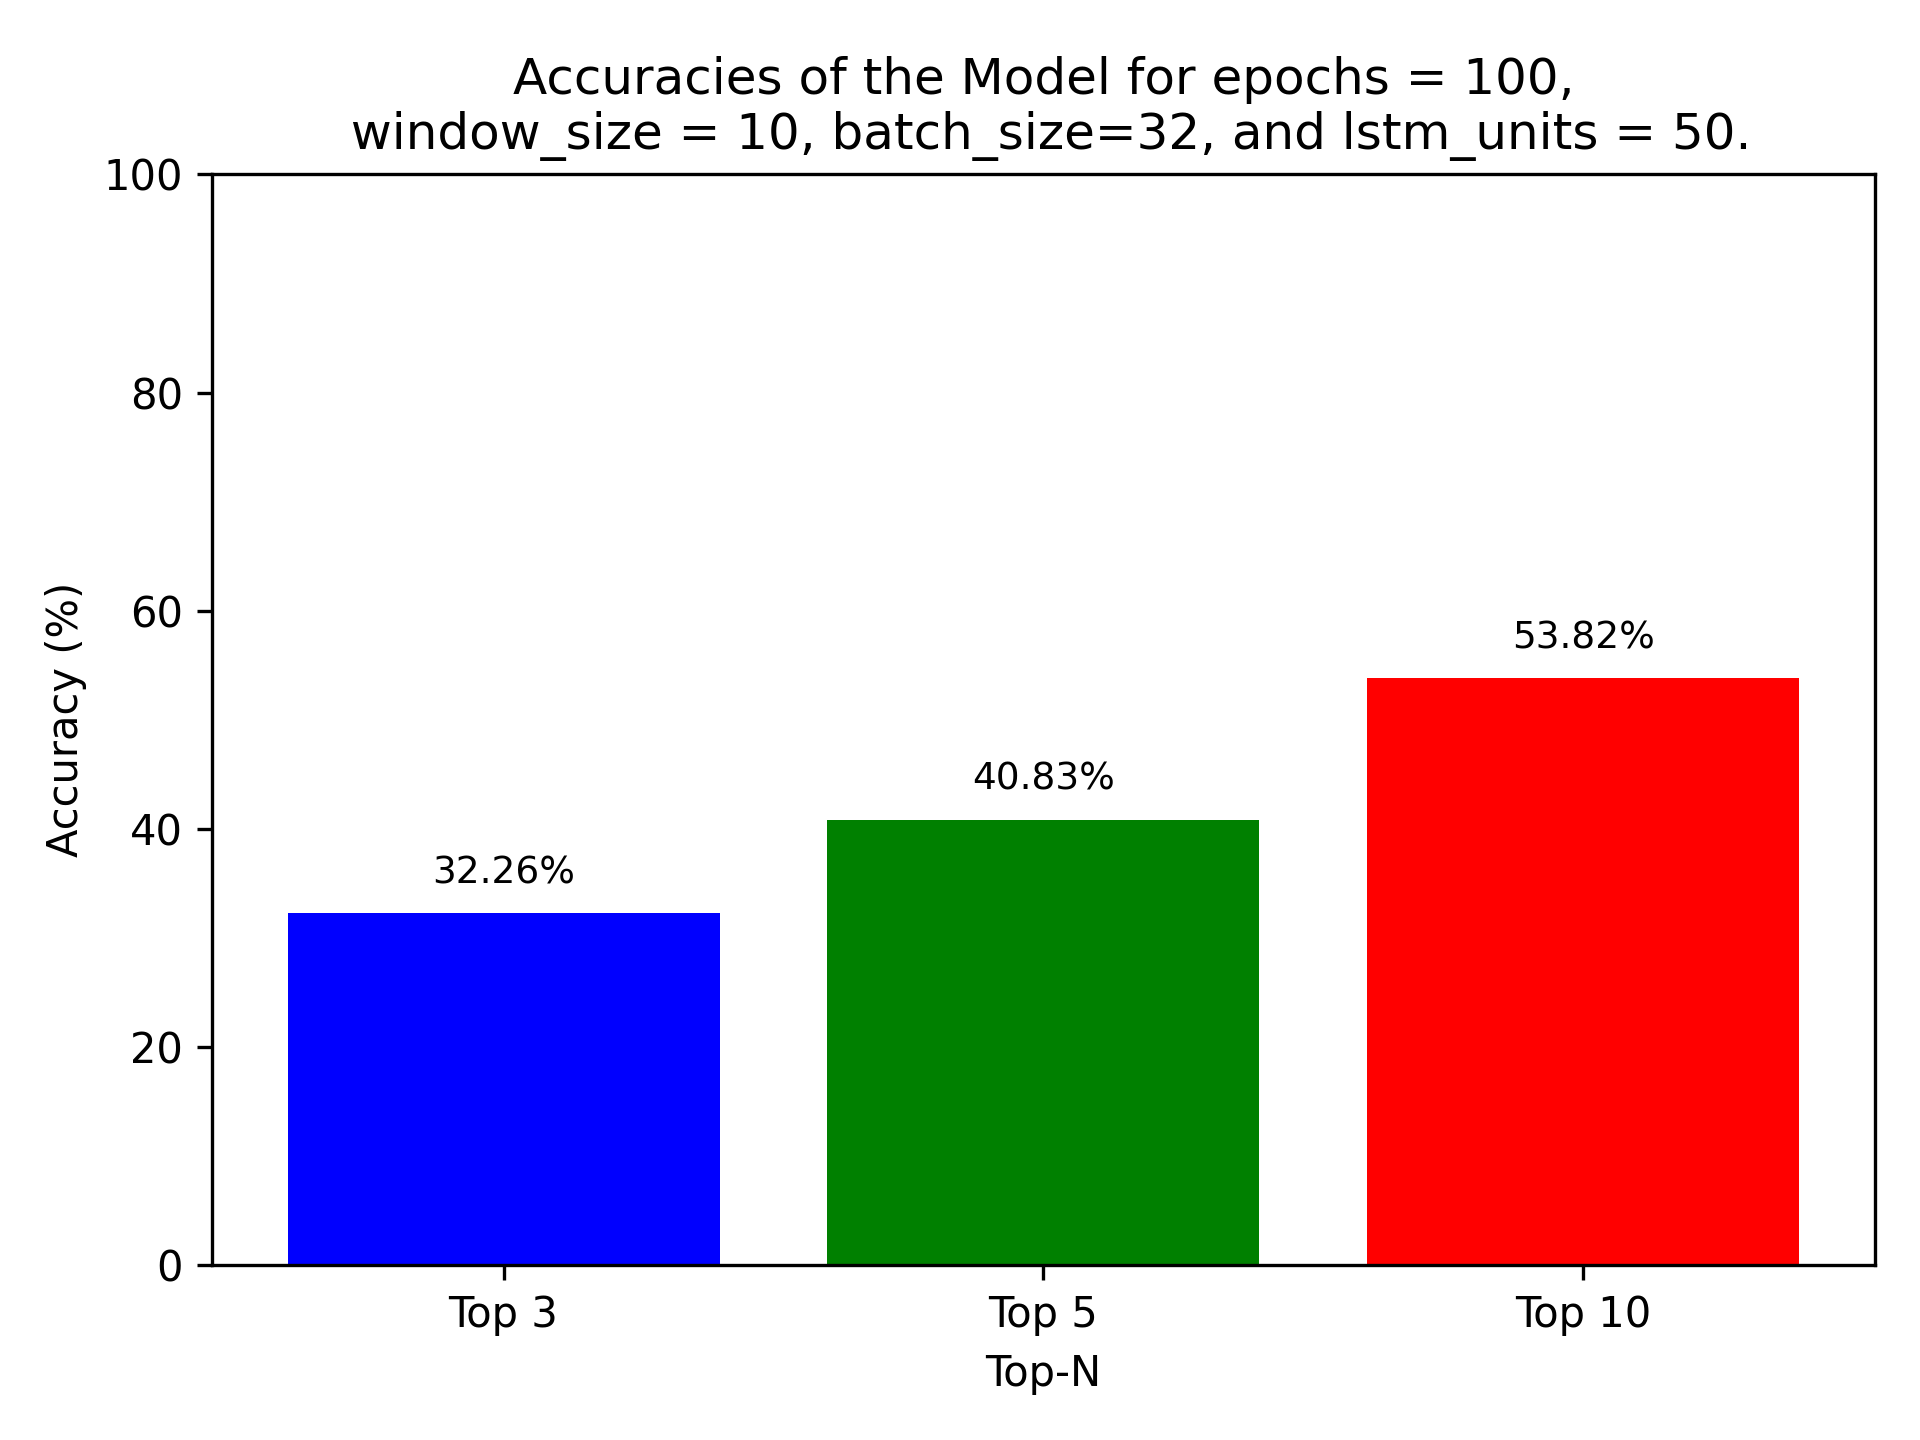
\includegraphics[scale=0.5]{images/accuracy_epochs_100_window_10_batch_32_lstm_50.png}
    \end{subfigure}

    \vspace{3em}

    \begin{subfigure}[b]{0.45\textwidth}
        \centering
        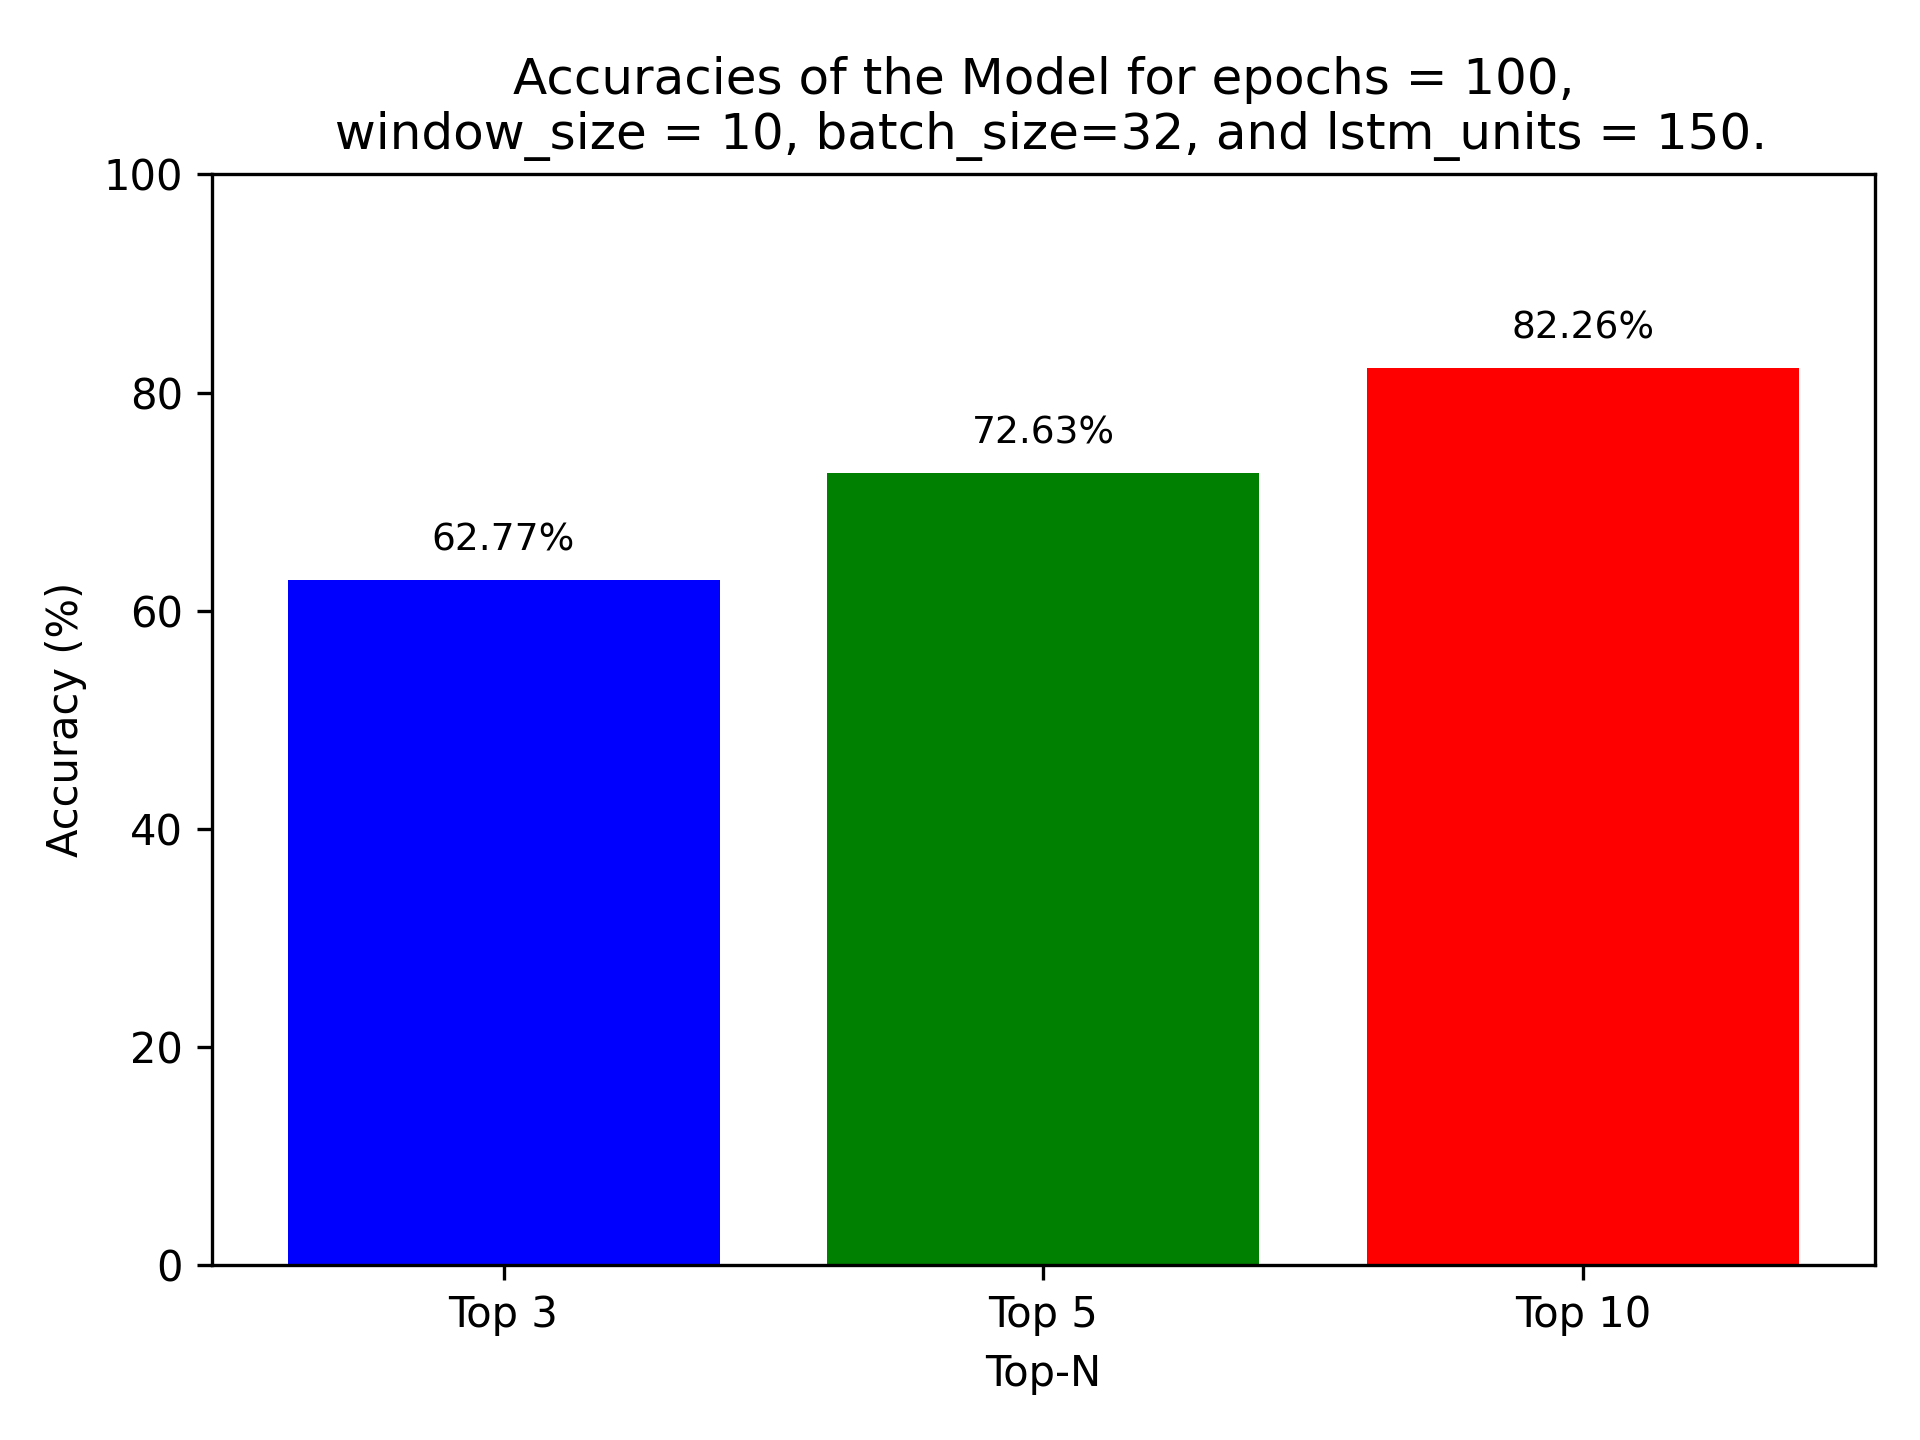
\includegraphics[scale=0.5]{images/accuracy_epochs_100_window_10_batch_32_lstm_150.png}
    \end{subfigure}
    \hfill
    \begin{subfigure}[b]{0.45\textwidth}
        \centering
        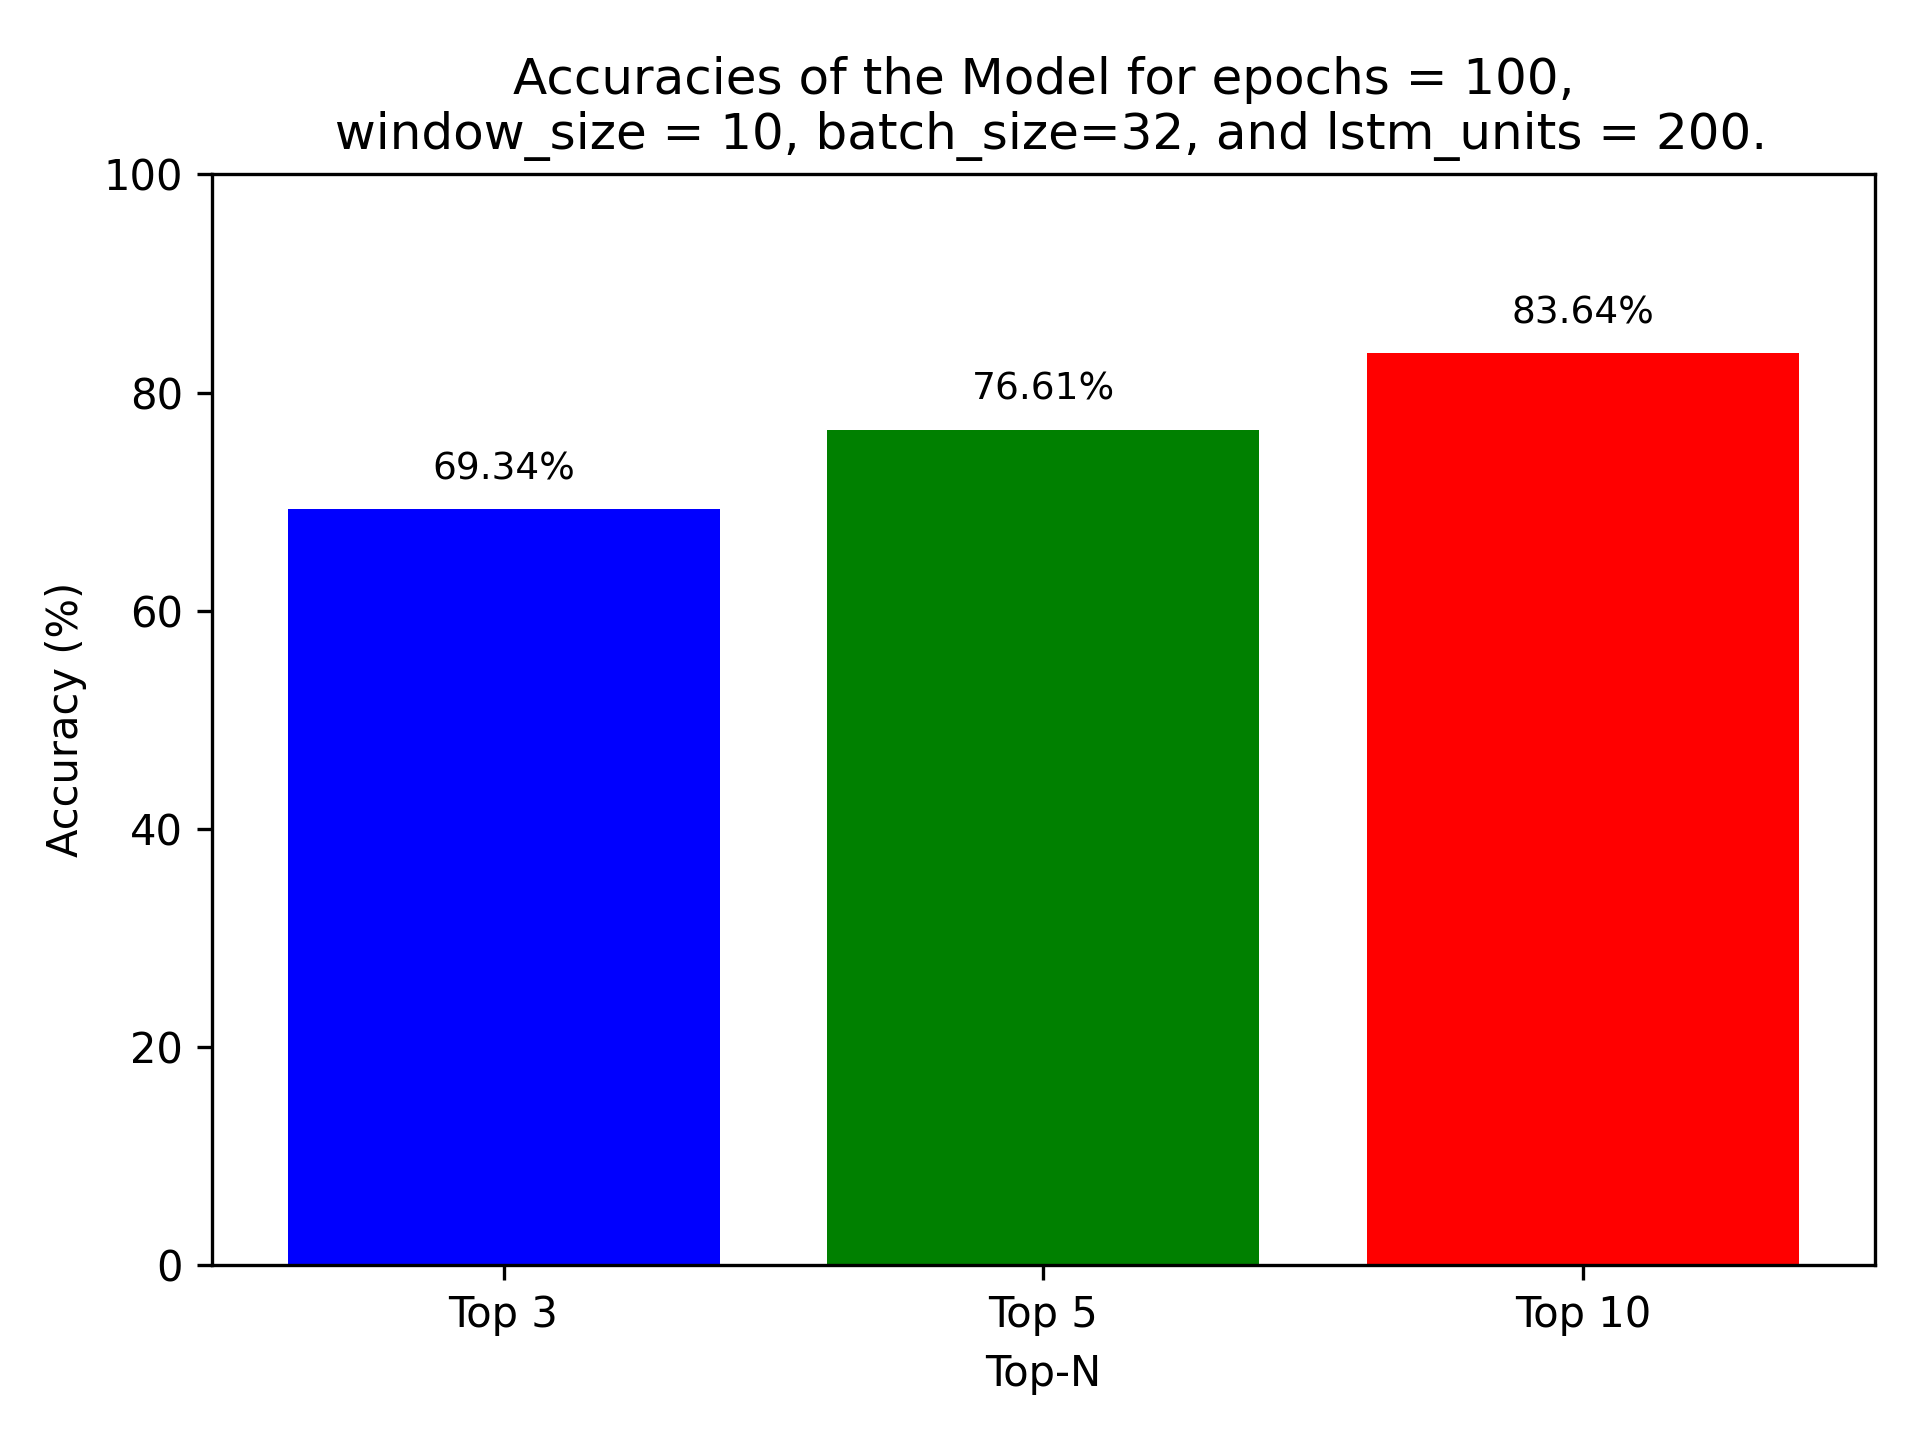
\includegraphics[scale=0.5]{images/accuracy_epochs_100_window_10_batch_32_lstm_200.png}
        %\label{fig:accuracy_epochs_100_window_10_batch_32_lstm_50}
    \end{subfigure}


    \caption{Accuracy of the LSTM model with 100 epochs, window size of 10, batch size of 32 and {50, 100, 150, 200, 500 and 1000} units in the LSTM layer.}
    \label{fig:accuracy_epochs_100_window_10_batch_32_lstm_x}
\end{figure}



\begin{itemize}
    \item Comparison with random selection of classes: lstm better than random selection
    \item best performance: xx\%, see \cref{fig:accuracy_epochs_100_window_10_batch_32_lstm_x}
\end{itemize}

%\noindent
